\chapter{A insanidade das reservas fracionadas}
\label{les:13}

\begin{chapquote}{Lewis Carroll, \textit{Alice no País das Maravilhas}}
Era muito tarde para desejar isso! Ela continuou crescendo e crescendo, e logo precisou ajoelhar-se no chão. Em outro minuto não havia nem mesmo um quarto para isso, e ela tentou deitar-se com um cotovelo contra a porta e o outro braço sobre a cabeça! Alice continuava a crescer e, como último recurso, ela colocou um braço para fora da janela e um pé para dentro da chaminé, dizendo para si mesma 
\enquote{Agora eu não posso fazer mais nada, o que quer quer seja que aconteça. O que vai ser de mim?}
\end{chapquote}

Valor e dinheiro não são tópicos triviais, especialmente nos dias atuais. O processo de criação de dinheiro em nosso sistema bancário não é algo simples também, e não consigo afastar a sensação de que isso é assim propositalmente. O que eu encontrei anteriormente apenas dentro da faculdade e em textos jurídicos parece ser uma prática comum no mundo financeiro também: nada é explicado em termos simples para o público leigo, não porque é algo realmente complexo, mas porque a verdade está escondida atrás de camadas e camadas de jargões e complexidades \textit{aparentes}. \enquote{Política monetária expansionista, flexibilização quantitativa, estímulo fiscal à economia.} O público acena concordando, hipnotizado pelas palavras bonitas.

Um banco de reservas fracionárias e flexibilização quantitativa são duas dessas palavras fantasiosas, que ofuscam o que realmente está acontecendo, mascarando-o como algo complexo e difícil de entender. Se você explicasse a uma criança de cinco anos, a insanidade de ambos, tudo se tornaria aparente rapidamente.

Godfrey Bloom, dirigindo-se ao Parlamento Europeu durante um debate conjunto, disse isso de uma maneira mil vezes melhor do que eu posso dizer:

\begin{quotation}\begin{samepage}
\enquote{[...] você não entende direito o conceito de banco. Todos os bancos estão falidos. O Banco Santander, o Deutsche Bank, o Royal Bank of Scotland --- estão todos falidos! E por que eles estão falidos? Não é um ato de Deus. Não é algum tipo de tsunami. Eles estão falidos porque temos um sistema chamado 'banco de reserva fracionária', o que significa que os bancos podem emprestar dinheiro que na verdade não têm! É um escândalo criminoso e já dura muito tempo. [...] Temos falsificação --- às vezes chamada de afrouxamento quantitativo --- mas falsificação com qualquer outro nome. A impressão artificial de dinheiro que, se qualquer pessoa comum fizesse, iria para a prisão por muito tempo [...] e até começarmos a enviar banqueiros --- e eu incluo banqueiros centrais e políticos --- para a prisão para este ultraje, ele vai continuar.}
\begin{flushright} -- Godfrey Bloom\footnote{Debate conjunto na união bancária~\cite{godfrey-bloom}}
\end{flushright}\end{samepage}\end{quotation}

Deixe-me repetir a parte mais importante: os bancos podem emprestar dinheiro que na verdade não possuem.

Graças ao banco de reservas fracionárias, um banco só precisa manter uma pequena \textit{fração} de cada dólar que recebe. É algo entre $0$ e $10\%$, geralmente na extremidade inferior, o que torna as coisas ainda piores.

Vamos usar um exemplo concreto para entender melhor essa ideia maluca: Vamos usar a fração de $10\%$ para conseguirmos fazer todos os cálculos em nossa cabeça. Pense comigo, se você levar \$100 para um banco --- porque você não quer guardá-lo embaixo do seu colchão --- eles só precisam manter a \textit{fração} acordada. Em nosso exemplo, seria \$10, porque 10\% de \$100 é \$10. Simples, certo?

Então, o que os bancos fazem com o resto do dinheiro? O que acontece com o seus \$90? Eles fazem o que os bancos fazem, eles emprestam para outras pessoas. O resultado é um efeito multiplicador de moeda, que aumenta enormemente a oferta de moeda na economia (Figura ~\ref{fig:money-multiplier}). Seu depósito inicial de \$100 logo se transformará em \$190. Ao emprestar uma fração de 90\% dos \$90 recém-criados, logo teremos \$271 na economia. E \$343,90 depois disso. A oferta de dinheiro está aumentando recursivamente, uma vez que os bancos estão literalmente emprestando dinheiro que eles não possuem ~\cite{wiki:money-multiplier}. Sem um único Abracadabra, os bancos transformam magicamente \$100 em mil dólares ou mais. Acontece que multiplicar em 10x é fácil. Leva apenas algumas rodadas de empréstimo.

\begin{figure}
  \centering
  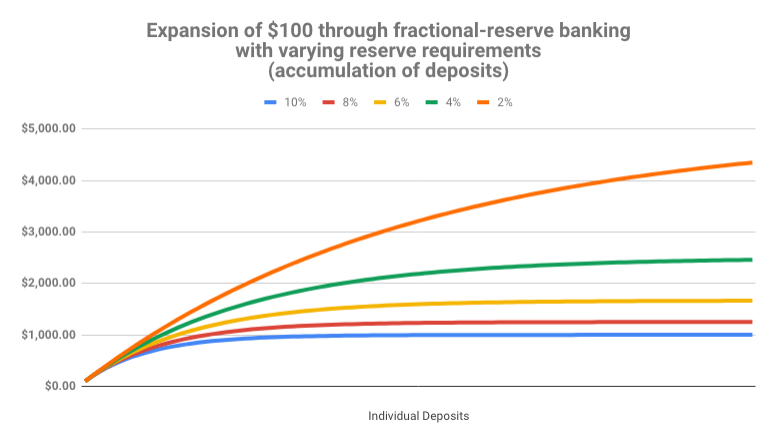
\includegraphics{assets/images/money-multiplier.png}
  \caption{O efeito multiplicador da moeda}
  \label{fig:money-multiplier}
\end{figure}

\paragraph{}
Não me entenda mal: não há nada de errado em fazer empréstimos. Não há nada de errado com os juros. Não há nada de errado com os bons e velhos bancos padrões que armazenavam sua fortuna em algum lugar mais seguro do que a sua gaveta de meias.

Os bancos centrais, no entanto, são uma besta diferente. Abominações de regulação financeira, metade pública metade privada, o fato de brincarem de deus com algo que afeta todos que fazem parte da nossa civilização global, sem consciência, apenas interessados no futuro imediato, e aparentemente sem qualquer responsabilidade ou auditoria (ver Figura~\ref{fig:bsg}).

\begin{figure}
  \centering
  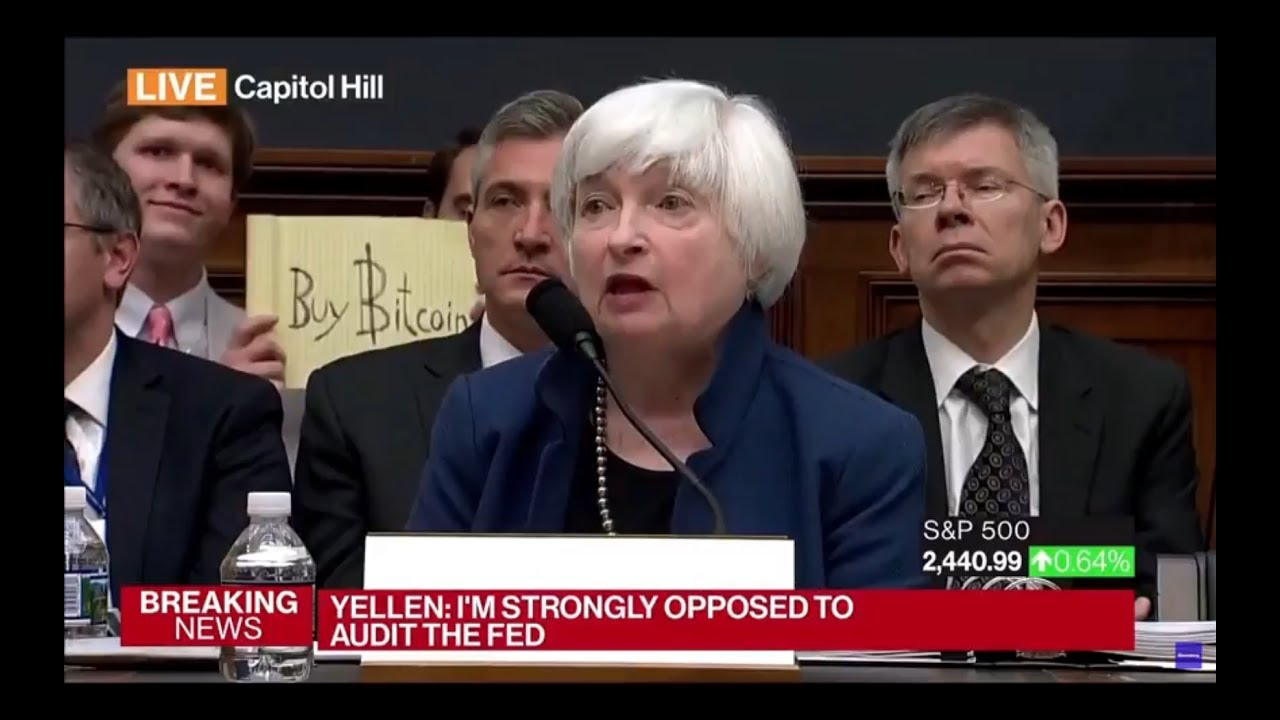
\includegraphics{assets/images/bsg.jpg}
  \caption{Yellen se opõe fortemente contra a auditoria do Fed, enquanto o Cara da Placa do Bitcoin é fortemente a favor de se comprar bitcoin.}
  \label{fig:bsg}
\end{figure}

Embora o Bitcoin ainda seja inflacionário, deixará de sê-lo em breve. O fornecimento estritamente limitado de 21 milhões de bitcoins acabará com a inflação por completo. Agora temos dois mundos monetários: um inflacionário, onde o dinheiro é impresso arbitrariamente, e o mundo do Bitcoin, onde o suprimento máximo é fixo e facilmente auditável por todos. Um é forçado através da violência, o outro pode ser acompanhado por qualquer um que queira. Sem barreiras de entrada, ninguém para pedir permissão. Uma participação voluntária. Essa é a beleza do Bitcoin.

\newpage

Eu diria que o argumento entre economistas keynesianos\footnote{Teorias monetárias que estão de acordo com John Maynard Keynes e seus discípulos ~\cite{wiki:keynesian}} e austríacos\footnote{Escola de pensamento econômico baseado no individualismo metodológico ~\cite{wiki:austrian}} não é apenas acadêmico.Satoshi conseguiu construir um sistema de transferência de valor com esteroides, criando o dinheiro mais forte que já existiu no processo. De uma forma ou de outra, mais e mais pessoas aprenderão sobre o golpe que é o banco de reservas fracionárias. Se chegarem a conclusões semelhantes às da maioria dos austríacos e dos bitcoinheiros, eles podem entrar na crescente Internet do dinheiro. Ninguém pode detê-los se decidirem fazer isso.

\paragraph{Bitcoin me ensinou que o banco de reservas fracionárias é pura insanidade.}

% ---
%
% #### Down the Rabbit Hole
%
% - [The Creature From Jekyll Island] by G. Edward Griffin
% - [Money Multiplier][money multiplier], [Keynesian Economics][Keynesian], [Austrian School][Austrian] on Wikipedia
%
% [The Creature From Jekyll Island]: https://archive.org/details/pdfy--Pori1NL6fKm2SnY
%
% [joint debate]: https://www.youtube.com/watch?v=hYzX3YZoMrs
% [money multiplier]: https://en.wikipedia.org/wiki/Money_multiplier
% [auditability]: https://i.ytimg.com/vi/ThFGs347MW8/maxresdefault.jpg
% [Keynesian]: https://en.wikipedia.org/wiki/Keynesian_economics
% [Austrian]: https://en.wikipedia.org/wiki/Austrian_School
%
% <!-- Wikipedia -->
% [alice]: https://en.wikipedia.org/wiki/Alice%27s_Adventures_in_Wonderland
% [carroll]: https://en.wikipedia.org/wiki/Lewis_Carroll
